\documentclass[border=20pt]{standalone}
\usepackage[utf8]{inputenc}
\usepackage{tikz}
\usetikzlibrary{calc, positioning}
\usepackage{amssymb}

\begin{document}
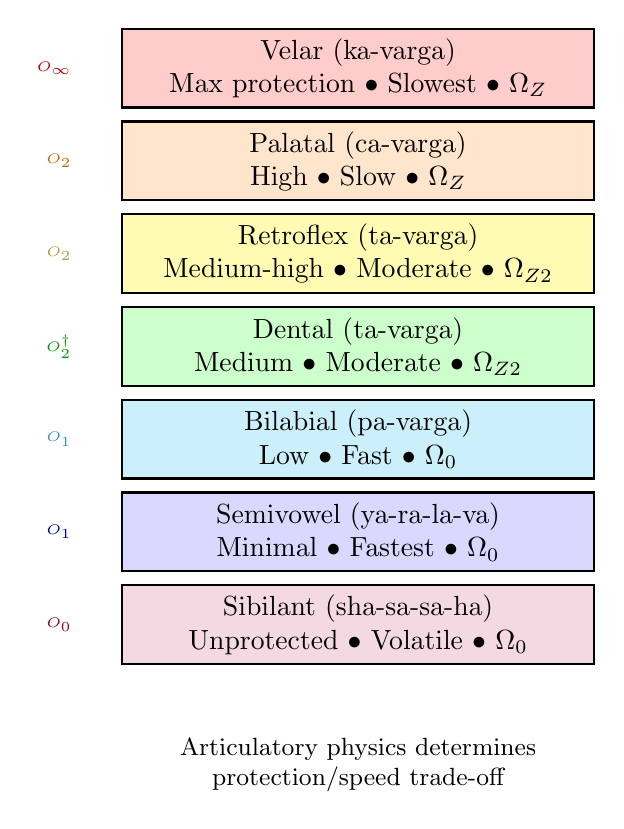
\begin{tikzpicture}[
  tier/.style={rectangle, draw, thick, minimum width=6cm, minimum height=1cm, align=center}
]
  \node[tier, fill=red!20] (velar) at (0,4) {Velar (ka-varga)\\Max protection $\bullet$ Slowest $\bullet$ $\Omega_Z$};
  \node[tier, fill=orange!20, below=0.15cm of velar] (palatal) {Palatal (ca-varga)\\High $\bullet$ Slow $\bullet$ $\Omega_Z$};
  \node[tier, fill=yellow!30, below=0.15cm of palatal] (retroflex) {Retroflex (ta-varga)\\Medium-high $\bullet$ Moderate $\bullet$ $\Omega_{Z2}$};
  \node[tier, fill=green!20, below=0.15cm of retroflex] (dental) {Dental (ta-varga)\\Medium $\bullet$ Moderate $\bullet$ $\Omega_{Z2}$};
  \node[tier, fill=cyan!20, below=0.15cm of dental] (bilabial) {Bilabial (pa-varga)\\Low $\bullet$ Fast $\bullet$ $\Omega_0$};
  \node[tier, fill=blue!15, below=0.15cm of bilabial] (semivowel) {Semivowel (ya-ra-la-va)\\Minimal $\bullet$ Fastest $\bullet$ $\Omega_0$};
  \node[tier, fill=purple!15, below=0.15cm of semivowel] (sibilant) {Sibilant (sha-sa-sa-ha)\\Unprotected $\bullet$ Volatile $\bullet$ $\Omega_0$};

  \node[below=0.8cm of sibilant, align=center, font=\small] {Articulatory physics determines\\protection/speed trade-off};

  % Left annotations
  \node[left=0.5cm of velar, font=\tiny\bfseries, text=red!70!black] {$O_{\infty}$};
  \node[left=0.5cm of palatal, font=\tiny\bfseries, text=orange!80!black] {$O_2$};
  \node[left=0.5cm of retroflex, font=\tiny\bfseries, text=yellow!60!black] {$O_2$};
  \node[left=0.5cm of dental, font=\tiny\bfseries, text=green!60!black] {$O_2^\dagger$};
  \node[left=0.5cm of bilabial, font=\tiny\bfseries, text=cyan!70!black] {$O_1$};
  \node[left=0.5cm of semivowel, font=\tiny\bfseries, text=blue!60!black] {$O_1$};
  \node[left=0.5cm of sibilant, font=\tiny\bfseries, text=purple!70!black] {$O_0$};
\end{tikzpicture}
\end{document}
